\documentclass[10pt]{article}

\usepackage[T1]{fontenc}
\usepackage{geometry}
\usepackage{amsmath, amssymb, amsthm}
\usepackage[scr]{rsfso}
\usepackage{graphicx}

\geometry{a4paper, margin=1in}

\renewcommand{\labelenumi}{(\roman{enumi})}

\newcounter{prob}
\newcommand{\problem}{\stepcounter{prob}\paragraph{Exercise \arabic{prob}}}
\newcommand{\solution}{\paragraph{Solution}}

\newcommand{\C}{\mathbb{C}}
\newcommand{\R}{\mathbb{R}}
\newcommand{\Q}{\mathbb{Q}}
\newcommand{\Z}{\mathbb{Z}}
\newcommand{\N}{\mathbb{N}}

\title{MA3103: Introduction to Graph Theory and Combinatorics}
\author{Satvik Saha}
\date{}

\begin{document}
    \noindent\textbf{IISER Kolkata} \hfill \textbf{Assignment II}
    \vspace{3pt}
    \hrule
    \vspace{3pt}
    \begin{center}
    \LARGE{\textbf{MA3101 : Introduction to Graph Theory and Combinatorics}}
    \end{center}
    \vspace{3pt}
    \hrule
    \vspace{3pt}
    Satvik Saha, \texttt{19MS154} \hfill \today
    \vspace{20pt}

    \problem Show that $R(2, k) = k$ for all $k \geq 2$.

    \solution Consider a colouring of the edges of $R(2, k)$ in red and blue. There
    are two possibilities: there exists a red edge $\{x, y\}$, or all edges are blue.
    In the former case, $x, y$ form a red $K_2$; in the latter case, the entire graph
    is itself a blue $K_k$.

    \problem Show that $R(3, 3, 3) \leq 17$.

    \solution Use Exercise 5 and $R_2(3) = R(3, 3) = 6$ to write $R_3(3) \leq (6 -
    1)\cdot 3 + 2 = 17$.

    \problem Draw a regular graph on 8 vertices such that it does not have a $K_3$,
    and an independent set of cardinality 4.

    \solution 

    \begin{center}
        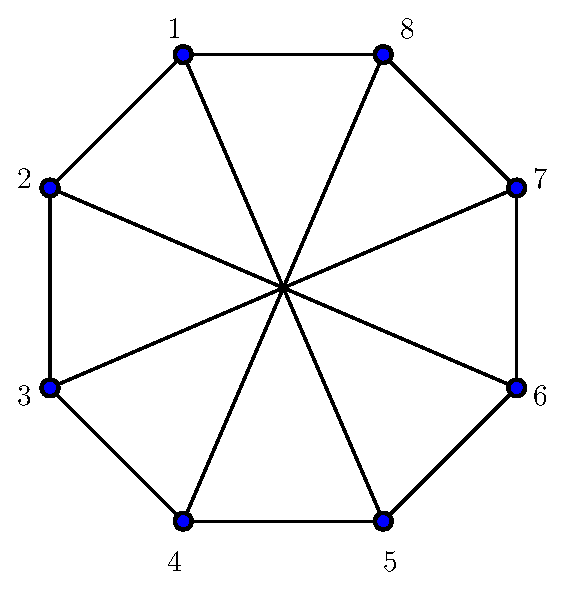
\includegraphics[width=0.45\textwidth]{./octagon_diags.eps}
    \end{center}

    Each vertex has degree $3$. It is clear by inspection that this is triangle free
    (the symmetry of the graph makes this easy to see).

    Suppose that this graph contains an independent set of size $4$, and without loss
    of generality suppose that this set contains the vertex $1$. This is directly
    connected to vertices $2, 5, 9$. Thus, the remaining three elements must be
    chosen from $\{3, 4, 7, 8\}$. However, at most one vertex can be chosen from
    each of the pairs $\{3, 7\}$ and $\{4, 8\}$ (they form edges), which makes our
    choice of an independent set of size $4$ impossible.

    \problem In case $R(m - 1, n)$ and $R(m, n - 1)$ are both even, prove that $R(m,
    n) \leq R(m - 1, n) + R(m, n - 1) - 1$.

    \problem The Ramsey number $R_k(3)$ is the minimum number $r$ of vertices such
    that, if the edges of $K_k$ are coloured with $k$ colours, there is always a
    monochromatic triangle. Now, show that for $n = (R_{k - 1}(3) - 1) \cdot k + 2$,
    if the edges of $K_n$ are coloured with $k$ colours, there is always a
    monochromatic triangle.

    \solution Consider an $r$ colouring of the edges of $K_n$, and fix a vertex $x$.
    Define the sets of vertices $A_i$, $1 \leq i \leq k$, such that each $A_i$
    consists of the neighbours of $x$ connected to it by an edge of colour $i$.
    Clearly, all $A_i$ are disjoint, and together they contain $n - 1 = (R_{k - 1}(3)
    - 1) \cdot k + 1$ vertices. Thus, the Strong Pigeonhole Principle guarantees that
    there is some colour, say $j$, such that $|A_j| \geq R_{k - 1}(3)$. Now, if the
    graph induced by $A_j$ contains an edge $\{y, z\}$ of colour $j$, then we have
    found a monochromatic triangle (colour $j$), namely $x, y, z$. Otherwise, $A_j$
    contains edges of only $k - 1$ colours, thus $|A_j| \geq R_{k - 1}(3)$ guarantees
    the existence of a monochromatic triangle. In either case, we are done.

    \problem Show that $R(s, t) > (s - 1)(t - 1)$.

    \solution Consider a graph $G$ on $(s - 1)(t - 1)$ vertices, which consists of $s
    - 1$ disconnected copies of $K_{t - 1}$. It is clear that $G$ contains neither an
    independent set of size $s$, nor a $t$-clique. This is because of the Pigeonhole
    Principle: given any $s$ vertices, at least two of them must belong to the same
    copy of $K_{t - 1}$ (of which there are $s - 1$), hence the set is not
    independent. Again, given any $t$ vertices, not all of them can belong to the
    same copy of $K_{t - 1}$ (each of which contains only $t - 1$ vertices), hence
    this is not a $t$-clique.

    Note that in our construction, $G$ is a complete $(t - 1)$-partite graph with $s
    - 1$ vertices in each part.

    \problem If $n$ is a positive integer satisfying \[
        \binom{n}{s} < 2^{\binom{s}{2} - 1},
    \] then show that $R(s, s) > n$.

    \solution We show that there is a 2-colouring of the edges of $K_n$ such that it
    contains no monochromatic $K_s$. To do this, we count the number of ways a $K_n$
    can contain a monochromatic $K_s$, and show that this is strictly less than the
    total number of colourings of $K_n$; the remaining colourings are thus free of a
    monochromatic $K_s$.

    First, note that $K_n$ contains $\binom{n}{2}$ edges, hence the total number of
    2-colourings of $K_n$ are \[
        2^{\binom{n}{2}}.
    \] Now, consider a $K_s \subset K_n$, which can be chosen in $\binom{n}{s}$ ways.
    For this to be monochromatic, there are two ways of colouring its edges (say red
    or blue). The number of remaining edges is $\binom{n}{2} - \binom{s}{2}$. Note
    that we have over-counted the total number of colourings with a monochromatic
    $K_s$, but this is not an issue: the number of such configurations is at most \[
        \binom{n}{s}\cdot 2\cdot 2^{\binom{n}{2} - \binom{s}{2}}.
    \] To show that this falls short of all colourings, it is sufficient to prove \[
        \binom{n}{s}\cdot 2\cdot 2^{\binom{n}{2} - \binom{s}{2}} < 2^{\binom{n}{2}},
        \qquad
        \binom{n}{s} < 2^{\binom{s}{2} - 1}.
    \] This is exactly what was given, completing the proof.

    \problem $S(r)$ is called Schur's number if it is the smallest integer such that
    any $r$ colouring of the integers $\{1, 2, \dots, S(r)\}$ contains three
    monochromatic integers $x, y, z$ such that $z = x + y$. Now, show that $S(r + 1)
    \geq 3S(r) - 1$.

    \solution Set $n = S(r) - 1$. Thus, there exists an $r$ colouring of $\{1, \dots,
    n\}$, say $\mathscr{C}$, such that no three monochromatic integers satisfy $x + y
    = z$. We shall construct an $r + 1$ colouring $\mathscr{C}'$ of $\{1, 2, \dots,
    3n + 1\}$ such that the integer sum property is still not satisfied; this is
    enough to show that $S(r + 1) > 3n + 1 = 3S(r) - 2$.

    To do this, colour the first block $\{1, 2, \dots, n\}$ as in $\mathscr{C}$,
    i.e.\ $\mathscr{C}'(i) = \mathscr{C}(i)$ for $1 \leq i \leq n$. Also colour the
    last block $\{2n + 2, \dots, 3n + 1\}$ in the say way, i.e.\ $\mathscr{C}'(2n + 1
    + i) = \mathscr{C}(i)$ for $1 \leq i \leq n$. Colour the remaining block $\{n +
    1, \dots, 2n + 1\}$ in the new, $(r + 1)$th colour, i.e.\ $\mathscr{C}'(n + i) =
    r + 1$ for $1 \leq i \leq n + 1$.

    Suppose that $x, y, z \in \{1, 2, \dots, 3n + 1\}$ have the colour $r + 1$. Then,
    they must be in the middle block, so $x + y \geq n + 1 + n + 1 = 2n + 2$ but $z
    \leq 2n + 1$. Thus, no $(r + 1)$-coloured triple $x, y, z$ can satisfy $x + y =
    z$.

    Thus, if monochromatic $x, y, z$ satisfy $x + y = z$, then they must belong to
    the extreme blocks and cannot have the $(r + 1)$th colour. Without loss of
    generality, suppose $x \leq y < z$. If both $x$ and $y$ belong to the first
    block, then $x + y \leq n + n = 2n$, forcing $z$ to belong to the first block as
    well (the integers $\{n + 1, \dots, 2n\}$ are in the wrong colour). However, this
    is not possible by the construction of $\mathscr{C}$. Again, if both $x$ and $y$
    belong to the last block, then $x + y \geq 2n + 2 + 2n + 2 = 4n + 4 > 3n + 1$,
    making the choice of $z$ impossible.

    Thus, we must have $x$ in the first block and $y, z$ in the last block. Write $y
    = 2n + 1 + y'$, $z = 2n + 1 + z'$ where $1 \leq y', z' \leq n$. Then, $x + y = z$
    gives $x + y' = z'$, with $x, y', z' \in \{1, \dots, n\}$. Furthermore, we have
    $\mathscr{C}'(y) = \mathscr{C}(y')$, $\mathscr{C'}(z) = \mathscr{C}(z')$ by
    construction, so $x, y', z'$ are monochromatic. Again, this is not possible
    because by the construction of $\mathscr{C}$.

    \problem Using the above relation, show that $S(r) \geq (3^r + 1) / 2$.

    \solution We have seen by inspection that $S(1) = 2$, $S(2) = 5$, hence these
    base cases hold. Suppose that the desired inequality holds for some $r \geq 2$.
    Then, using the inequality from the previous exercise with the induction
    hypothesis, \[
        S(r + 1) \geq 3S(r) - 1 \geq 3\cdot \frac{3^r + 1}{2} - 1 = \frac{3^{r + 1} +
        1}{2}.
    \] This proves the desired result by induction.

    \problem For $r \geq 1$, show that there exists a smallest natural number $S'(r)$
    such that every $r$ colouring of the integers $\{1, 2, \dots, N\}$ with $N \geq
    S'(r)$ will necessarily contain three integers $x, y, z$ (all must not be the
    same) of the same colour such that $z = xy$.

    \solution Let $n = 2^{S(r)}$; we claim that $S'(r) \leq n$. Consider an arbitrary
    $r$ colouring of the integers $\{1, 2, \dots, n\}$; this gives an $r$ colouring
    of the subset $A = \{2^1, 2^2, \dots, 2^{S(r)}\}$. Again, this gives an $r$
    colouring of the integers $B = \{1, 2, \dots, S(r)\}$, by setting the colour of
    $k \in B$ to the colour of $2^k \in A$. Thus, we are guaranteed monochromatic
    $x', y', z' \in B$ such that $x' + y' = z'$. The corresponding elements $x =
    2^{x'}$, $y = 2^{y'}$, $z = 2^{z'} \in A$ are monochromatic, with $xy = z$.
    Furthermore, not all of them can be the same since $z' > x', y'$.

    \problem Can you construct graphs with the following degree sequences? Provide
    proper justifications.
    \begin{enumerate}
        \itemsep0em
        \item 5, 5, 4, 3, 2, 2, 2, 1
        \item 5, 5, 4, 4, 2, 2, 1, 1
        \item 5, 5, 5, 3, 2, 2, 1, 1
        \item 5, 5, 5, 4, 2, 1, 1, 1
    \end{enumerate}

    \solution We employ the Havel-Hakimi scheme, which involves arranging the
    sequence in descending order, removing $d_1$ and subtracting $1$ from the next
    $d_i$ numbers, then repeating.
    \begin{enumerate}
        \item \begin{align*}
            5, 5, 4, 3, 2, 2, 2, 1 \\
            4, 3, 2, 1, 1, 2, 1 \\
            4, 3, 2, 2, 1, 1, 1 \tag{Reorder} \\
            2, 1, 1, 0, 1, 1 \\
            2, 1, 1, 1, 1 \tag{Reorder} \\
            0, 0, 1, 1
        \end{align*}
        At this point, the sequence is clearly graphic: consider $K_2$ with $2$ extra
        isolated points. Thus, the initial sequence is also graphic.

        \item \begin{align*}
            5, 5, 4, 4, 2, 2, 1, 1 \\
            4, 3, 3, 1, 1, 1, 1 \\
            2, 2, 0, 0, 1, 1
        \end{align*}
        At this point, the sequence is clearly graphic: consider $P_4$ (a path of
        four vertices in a line) with $2$ extra isolated points. Thus, the initial
        sequence is graphic.
        
        \item \begin{align*}
            5, 5, 5, 3, 2, 2, 1, 1 \\
            4, 4, 2, 1, 1, 1, 1 \\
            3, 1, 0, 0, 1, 1
        \end{align*}
        At this point, the sequence is clearly graphic: consider $K_{1, 3}$ (a star
        with 3 points) with $2$ extra isolated points. Thus, the initial sequence is
        graphic.

        \item \begin{align*}
            5, 5, 5, 4, 2, 1, 1, 1 \\
            4, 4, 3, 1, 0, 1, 1 \\
            4, 4, 3, 1, 1, 1, 0 \tag{Reorder} \\
            3, 2, 0, 0, 1, 0
        \end{align*}
        At this point, the sequence is clearly not graphic: the first vertex has
        degree $3$ but there are only two remaining vertices of positive degree.
        Thus, the initial sequence is not graphic.

    \end{enumerate}

    \problem For each of the sequences of numbers below, explain why there cannot be
    any graph having that sequence.
    \begin{enumerate}
        \itemsep0em
        \item 5, 5, 5, 4, 4, 3, 3
        \item 6, 5, 4, 3, 2, 2, 0
    \end{enumerate}
    
    \solution   
    \begin{enumerate}
        \item Here, the sum of the degrees of the vertices is an odd number, which
        contradicts the fact that the sum ought to be $2|E|$ which is an even number.

        \item Here, the first vertex has degree $6$, but there are only $5$ remaining
        vertices with positive order.
    \end{enumerate} 

    \problem Can you construct graphs with the following degree sequences?
    Can you construct bipartite graphs from those graphic sequences?
    \begin{enumerate}
        \itemsep0em
        \item 5, 3, 3, 3, 2, 2, 2, 2, 2, 2
        \item 6, 6, 6, 4, 4, 4, 4, 4, 4, 4, 4, 4, 4
    \end{enumerate}

    \solution 
    \begin{enumerate}
        \item \begin{align*}
            5, 3, 3, 3, 2, 2, 2, 2, 2, 2 \\
            2, 2, 2, 1, 1, 2, 2, 2, 2
        \end{align*}
        This is clearly graphic: consider $P_9$ (a path of 9 vertices). A bipartite
        graph with the given degree sequence is given below.

        \begin{center}
            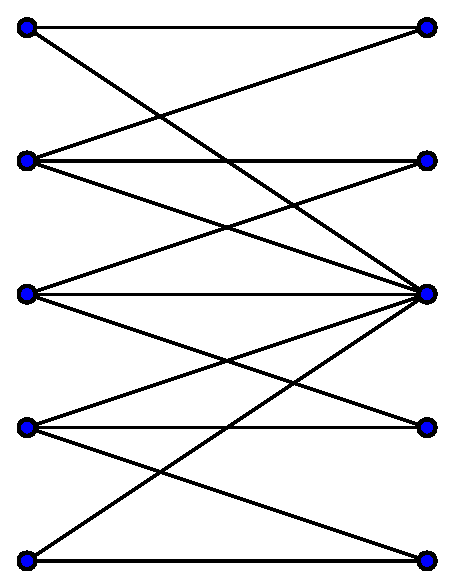
\includegraphics[width=0.4\textwidth]{./bipartite_13_1.eps}
        \end{center}

        \item \begin{align*}
            6, 6, 6, 4, 4, 4, 4, 4, 4, 4, 4, 4, 4 \\
            5, 5, 3, 3, 3, 3, 4, 4, 4, 4, 4, 4 \\
            5, 5, 4, 4, 4, 4, 4, 4, 3, 3, 3, 3 \tag{Reorder} \\
            4, 3, 3, 3, 3, 4, 4, 3, 3, 3, 3 \\
            4, 4, 4, 3, 3, 3, 3, 3, 3, 3, 3 \tag{Reorder} \\
            3, 3, 2, 2, 3, 3, 3, 3, 3, 3
        \end{align*}
        This is graphic. Divide the sequence into the parts $3, 3, 2, 2$ and $3, 3,
        3, 3, 3, 3$.
        
        \begin{center}
            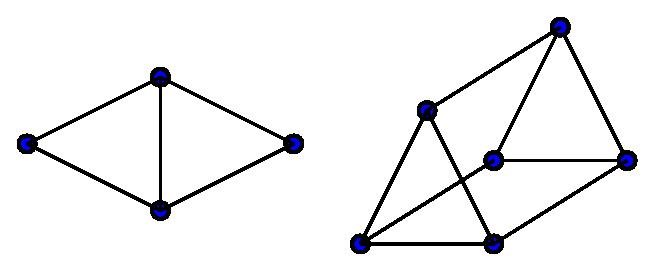
\includegraphics[width=0.6\textwidth]{./graph_13_2.eps}
        \end{center}
        
        Suppose that $G$ is a bipartite graph with the given degree sequence. The sum
        of the degrees is $6\cdot 3 + 4\cdot 10 = 58$, hence $G$ has exactly $29$
        edges. Since $G$ is bipartite, every edge connects a vertex from one part to
        the other. Thus, the total number of edges leaving one part is also $29$, and
        the sum of degrees of the vertices in that part is also $29$. This
        contradicts the fact that all vertices have even degree.
    \end{enumerate}

    \problem Show that a graph that has 17 vertices and 73 edges cannot be bipartite.

    \solution Calculate \[
        |E| = 73 > \left\lfloor \frac{n^2}{4}\right\rfloor = \left\lfloor
        \frac{17^2}{4} \right\rfloor = 72.
    \] Mantel's theorem guarantees the existence of a triangle in any such graph.
    However, a bipartite graph is always triangle-free.

    \problem If a sequence $(d_i)_1^n$ of non-negative integers such that $d_1 \geq
    d_2 \geq \dots \geq d_n$ is graphic, then show that for $1 \leq m \leq n$, \[
        \sum_{i = 1}^m d_i \;\leq\; m(m - 1) + \sum_{i = m + 1}^n \min(d_i, m).
    \]

    \solution Given a graph $G$ obeying this scheme, let $A = \{x_1, x_2, \dots,
    x_m\}$ be the set of $m$ vertices with the highest degrees, $d_1, d_2, \dots,
    d_m$, and let $B$ be the remaining vertices. Let $I(e, x)$ be the incidence
    function between edges and vertices. Let $F$ be the set of edges which have at
    both endpoints in $A$, and let $H$ be the set of edges with one endpoint in $A$,
    the other in $B$. Note that \[
        \sum_{i = 1}^m d_i = \sum_{x \in A} d(x) = \sum_{x \in A} \sum_{e \in F\cup
        H} I(e, x) = \sum_{e \in F \cup H} \sum_{x \in A} I(e, x) = \sum_{e \in F} 2
        + \sum_{e \in H} 1 = 2 |F| + |H|.
    \] This is because each $e \in F$ contributes $2$ to the sum via both endpoints,
    while each $e \in H$ contributes only $1$. We only need to consider edges with at
    least one endpoint in $A$.

    Now, clearly $|F| \leq \binom{m}{2} = m(m - 1) / 2$. To count the edges in $H$,
    pick a vertex $x \in B$. This can contribute at most $d(x)$ edges to the entire
    graph; at the same time, there are only $m$ vertices in $A$. Thus, $x$
    contributes at most $\min(d(x), m)$ edges to $H$. Summing over all vertices in
    $B$ and putting things together, \[
        \sum_{i = 1}^m d_i \;\leq\; 2|F| + |H| \;\leq\; m(m - 1) + \sum_{i = m + 1}^n
        \min(d_i, m).
    \] 

\end{document}
